%% template for IEICE Transactions
%% v2.1 [2015/10/31]
\documentclass[paper]{ieice}
%\documentclass[invited]{ieice}
%\documentclass[position]{ieice}
%\documentclass[survey]{ieice}
%\documentclass[invitedsurvey]{ieice}
%\documentclass[review]{ieice}
%\documentclass[tutorial]{ieice}
%\documentclass[letter]{ieice}
%\documentclass[brief]{ieice}
%\usepackage[dvips]{graphicx}
%\usepackage[pdftex]{graphicx,xcolor}
\usepackage[dvipdfmx]{graphicx,xcolor}
\usepackage[fleqn]{amsmath}
\usepackage{newtxtext}
\usepackage[varg]{newtxmath}
\usepackage{bm}
\usepackage{comment}

\setcounter{page}{1}
%\breakauthorline{}% breaks lines after the n-th author

\field{}
%\SpecialIssue{}
%\SpecialSection{}
%\theme{}
\title{Compactness of Finite Union of Regular Patterns and Regular Patterns without Adjacent Variables}
%\title[title for header]{title}
%\titlenote{}
\authorlist{%
\authorentry{Naoto Taketa}{n}{labelA}\MembershipNumber{0000000}
\authorentry{Tomoyuki Uchida}{m}{labelA}\MembershipNumber{9230354}
\authorentry{Takayoshi Shoudai}{m}{labelB}\MembershipNumber{9303359}
\authorentry{Satoshi Matsumoto}{m}{labelC}\MembershipNumber{0307572}
\authorentry{Yusuke Suzuki}{m}{labelA}\MembershipNumber{0120588}
\authorentry{Tetsuhiro Miyahara}{m}{labelA}\MembershipNumber{0401030}
%\authorentry{Takayoshi Shoudai}{m}{labelB}[present affiliate label]\MembershipNumber{}
% \authorentry[e-mail address]{name}{membership}{affiliate label}\MembershipNumber{}
% \authorentry[e-mail address]{name}{membership}{affiliate label}[present affiliate label]\MembershipNumber{}
}
\affiliate[labelA]{Graduate School of Information Sciences, Hiroshima City University}
\affiliate[labelB]{Department of Computer Science and Engineering, Fukuoka
Institute of Technology}
\affiliate[labelC]{Faculty of Science, Tokai University}
%\affiliate[affiliate label]{The author is with the 
%}
%\paffiliate[present affiliate label]{Presently, the author is with the }

\received{2015}{1}{1}
\revised{2015}{1}{1}

%% <local definitions here>
\newtheorem{dfn}{Definition} 
\newtheorem{thm}{Theorem}
\newtheorem{lem}{Lemma}
\newtheorem{col}{Corollary}
\newtheorem{ex}{Example}
\newtheorem{cl}{Claim}
\newenvironment{proof}{\noindent{\bf Proof.}}{\par\medskip}
\renewcommand{\labelenumi}{(\arabic{enumi})}
\newcommand{\proofname}{\textbf{Proof.}}
\newcommand{\qedsymbol}{(Q.E.D)}
%\newcommand{\L}{\mathcal{L}}
\newcommand{\Pat}{\mathcal{P}}
\newcommand{\RPat}{\mathcal{RP}}
\newcommand{\PatL}{\mathcal{P\!\!L}}
\newcommand{\RPatL}{\mathcal{RP\!\!L}}
\newcommand{\Patplus}{\Pat^{+}}
\newcommand{\RPatplus}{\RPat^{+}}
\newcommand{\Patkei}{\Pat^{k}}
\newcommand{\RPatkei}{\RPat^{k}}
\newcommand{\PatLkei}{\PatL^{k}}
\newcommand{\RPatLkei}{\RPatL^{k}}
\newcommand{\NAV}{N\!A\!V}
\newcommand{\NAVR}{\RPat_{N\!A\!V}}
\newcommand{\NAVRPplus}{\RPat^{+}_{N\!A\!V}}
\newcommand{\NAVRPkei}{\RPat^{k}_{N\!A\!V}}

%% </local definitions here>

\begin{document}

\begin{figure*}[t]
  \begin{center}
    %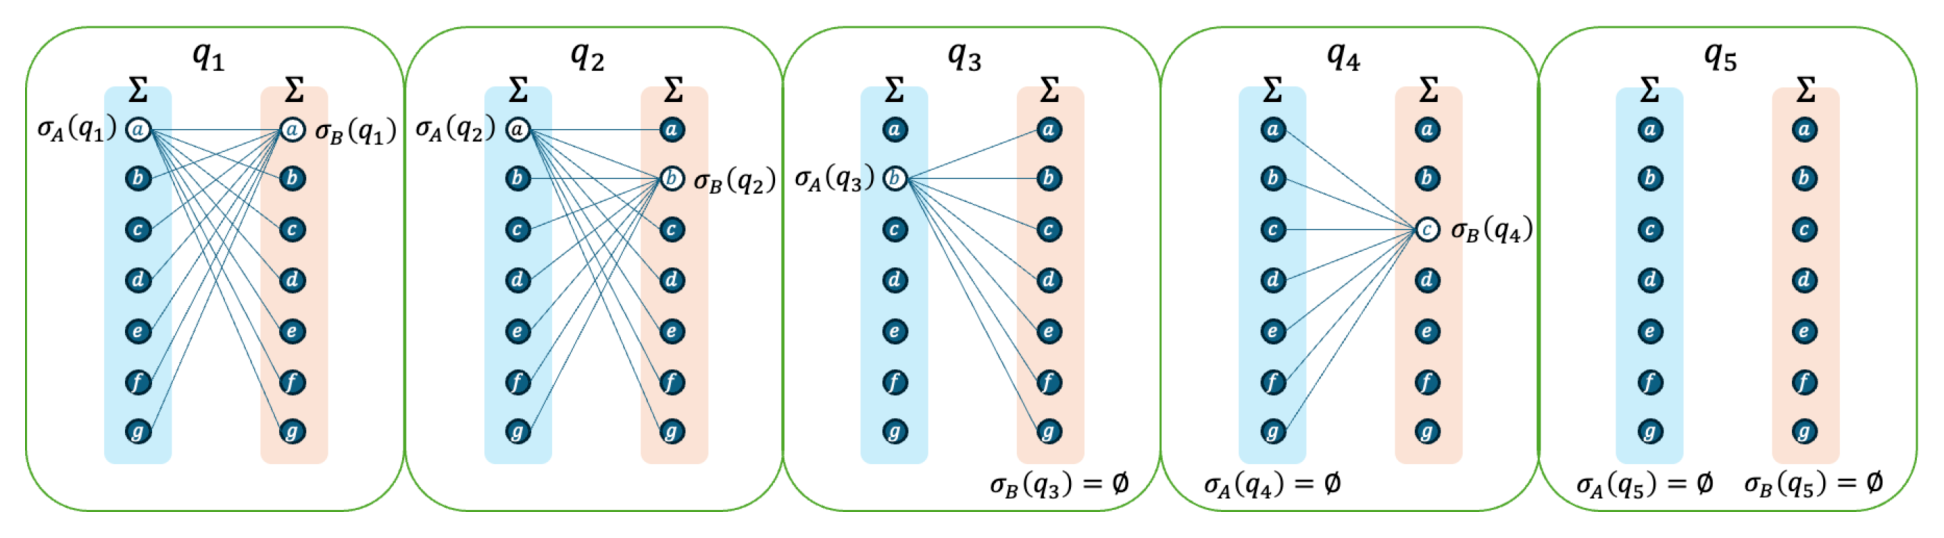
\includegraphics[scale=0.5]{figs/lem8eachreg.eps}
    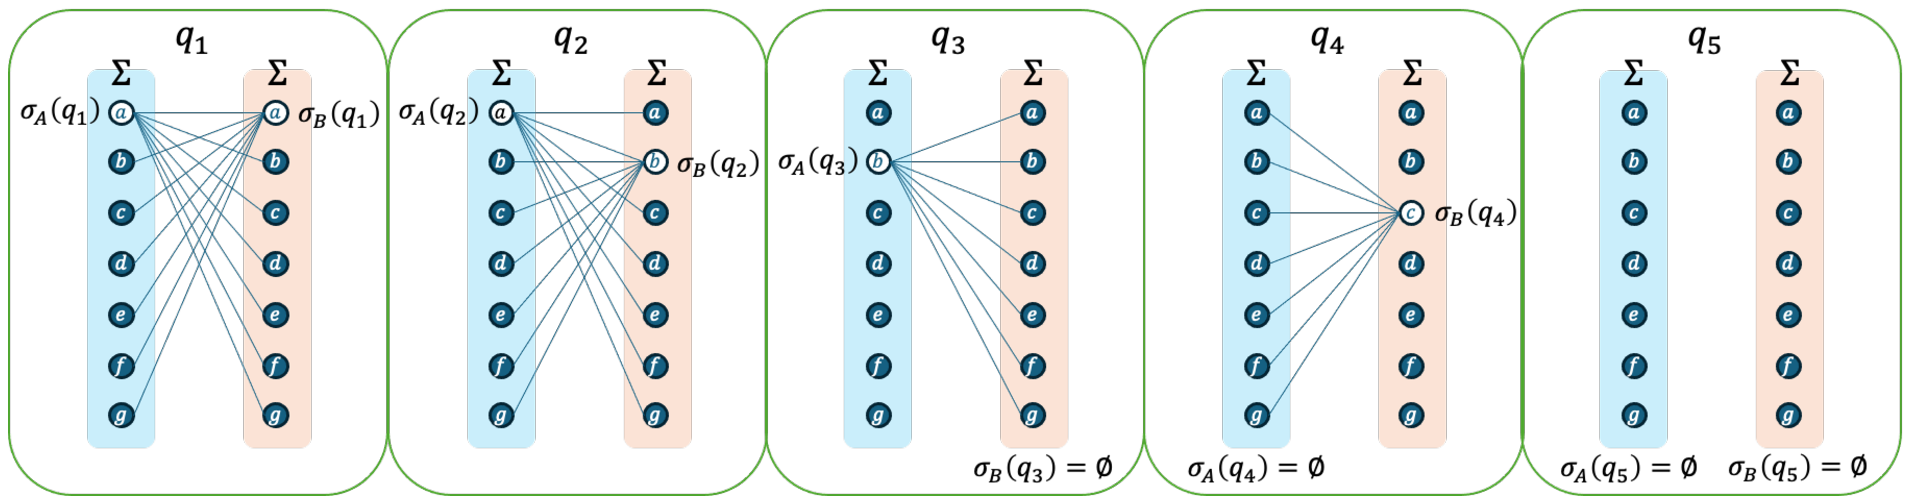
\includegraphics[scale=0.54]{figs/lem8eachreg.pdf}
    \caption{Let $\Sigma=\{a,b,c,d,e,f,g\}, Q=\{q_1,q_2,q_3,q_4,q_5\}$. We set $A(q_1)=\{a\}$ and $B(q_1)=\{a\}$, and then $\sigma_A(q_1)=a$ and $\sigma_B(q_1)=a$, and so on. For each regular pattern $q_i$ ($i=1,\ldots,5$), we represent a string $w \in \Sigma\cdot\Sigma$ satisfying that $p\{x:=w\}\preceq q_i$ by the edge between the left (first) and right (second) symbols of $w$. For example, the leftmost figure shows that $p\{x:=ay\}\preceq q_1$ and $p\{x:=ya\}\preceq q_1$ for a variable symbol $y$. We note that these figures may contain more edges than those illustrated. From these figures, we get $\ell_A=1, \ell_B=0$, and $Q^{(\bot,\bot)}=\{q_5\}, Q^{(\bot,\cdot)}=\{q_4\}, Q^{(\cdot,\bot)}=\{q_3\}, Q^{(\cdot,\cdot)}=\{q_1,q_2\}$.}\label{fig:lem8eachreg}
  \end{center}
\end{figure*}

\begin{figure}[t]
  \begin{center}
    %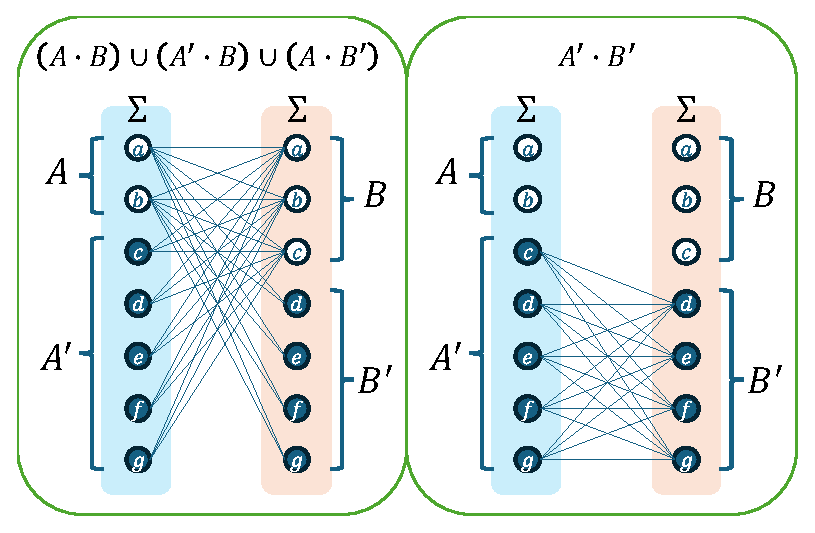
\includegraphics[scale=0.5]{figs/lem8totalreg.eps}
    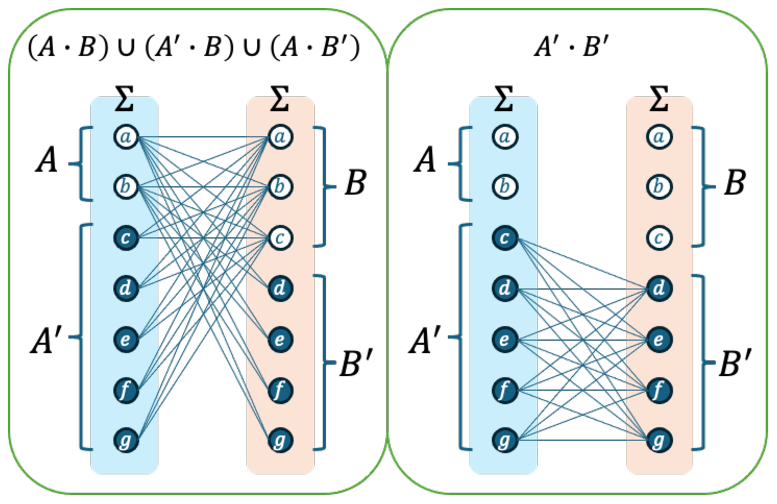
\includegraphics[scale=0.525]{figs/lem8totalreg.pdf}
    \caption{In the left figure, we aggregate all of the edges appearing in Fig.~\ref{fig:lem8eachreg}. For all $w=a'b'\in A'\cdot B'$, there must be a regular pattern $q_i$ $(1\leq i\leq 5$) that satisfies that $p \{ x:=w \} \preceq q_i$.}\label{fig:lem8totalreg}
  \end{center}
\end{figure}

\end{document}
